\documentclass[svgnames,unknownkeysallowed]{beamer}
\addtobeamertemplate{navigation symbols}{}{%
    \usebeamerfont{footline}%
    \usebeamercolor[fg]{footline}%
    \hspace{1em}%
    \insertframenumber/\inserttotalframenumber
}
\setbeamertemplate{section in toc}[sections numbered]
\setbeamertemplate{subsection in toc}[subsections numbered]
\usepackage{tikz}
\usepackage{xcolor}
\usepackage[utf8]{inputenc}
\usepackage{enumitem}
\usepackage{amsmath}
\usepackage{pifont}
\usepackage[figurename=]{caption}
\usepackage{pgfplots}
\usetikzlibrary{shapes.misc, positioning}
\usetikzlibrary{automata,matrix,backgrounds,mindmap,shadows}
\usepackage{tikz-er2}
\usepackage{bm}
\usepackage{graphicx}
\usepackage{pgf,pgfarrows,pgfnodes,pgfautomata,pgfheaps,pgfshade,pgfplots,picture,booktabs,array,multirow,picture}
\usetikzlibrary{arrows,fit,shapes,calc,patterns,calc,chains,positioning,shadows}
\usetikzlibrary{arrows,snakes,backgrounds,shapes,patterns,shadows,positioning,decorations.text,decorations.pathmorphing,matrix,calc,automata}
\usetikzlibrary{arrows}
\usepackage[normalem]{ulem}
\usepackage{pgfplots}
\usepgfplotslibrary{colorbrewer,groupplots}
\pgfplotsset{
compat=1.13,
cycle list/Set1-5,
cycle list/Set2,
cycle list/Set3
}
\usepackage{microtype}%if unwanted, comment out or use option "draft"
\usepackage{graphicx}
\definecolor{jungle}{RGB}{41,171,135}

\usepackage{pgf-pie}  

\usepackage{listings}
\DeclareCaptionFont{white}{\color{white}}
\DeclareCaptionFormat{listing}{\colorbox{gray}{\parbox{\textwidth}{#1#2#3}}}
\captionsetup[lstlisting]{format=listing,labelfont=white,textfont=white}


\usepackage{rtsched}

\input{python}

\title[Dresden] % (optional, only for long titles)
{Real-time scheduling of dynamic neural networks on multi-Edge TPU}
\title[Dresden] % (optional, only for long titles)
{Real-time scheduling of dynamic neural networks on multi-Edge TPU}
%\subtitle{Systèmes temps réel embarqués}
\author[Kłoda, Tomasz] % (optional, for multiple authors)
{Mouad Zouhdi, Jiahe Guo, Rafik Hammadi, Binqi Sun, ...}
\institute[Universities Here and There] % (optional)
{	
  LAAS-CNRS / Insa de Toulouse \\
  Toulouse, France
}
\date[Dresden2024] % (optional)
{Huawei 2012 Labs Global Software Technology Summit 2024\\\small Dresden 02.07.2024}
\subject{DDN real-time multi-TPU scheduling}


\AtBeginSection[]{
	\begin{frame}[noframenumbering]
		\vfill
		\centering { \Huge
		\begin{beamercolorbox}[sep=8pt,center,shadow=true,rounded=true]{title}
			\usebeamerfont{title}\insertsectionhead\par%
		\end{beamercolorbox} }
		\vfill
	\end{frame}
}


\begin{document}
% =====================================================================
%  Frames "benchmark" : les slides de resultats elagues.
%  A inserer dans presentation_dsd2026.tex par : % =====================================================================
%  Frames "benchmark" : les slides de resultats elagues.
%  A inserer dans presentation_dsd2026.tex par : % =====================================================================
%  Frames "benchmark" : les slides de resultats elagues.
%  A inserer dans presentation_dsd2026.tex par : \input{frames_benchmark}
%  Prerequis (deja dans le preambule) : pgfplots + groupplots, graphicx,
%  booktabs, tikz, xcolor.
%  Donnees : bench/data/*.csv       Images : bench/img/*
%  Les figures sont en pgfplots, meme rendu que les figures de l'article.
% =====================================================================

% --- palette des criteres d'importance (identique a celle de l'article) ---
\definecolor{impmagnitudel1}{HTML}{1F77B4}
\definecolor{impmagnitudel2}{HTML}{AEC7E8}
\definecolor{impbnscale}{HTML}{FF7F0E}
\definecolor{impfpgm}{HTML}{2CA02C}
\definecolor{imptaylor}{HTML}{D62728}
\definecolor{impobdc}{HTML}{9467BD}
\definecolor{imprandom}{HTML}{7F7F7F}

% --- style commun a tous les panneaux ---
\pgfplotsset{
  benchpanel/.style={
    grid=both, grid style={dashed,gray!30},
    tick label style={font=\scriptsize},
    label style={font=\scriptsize},
    title style={font=\small},
  },
  benchcurves/.style={mark=none, line width=1.0pt, unbounded coords=jump},
}

% --- legende partagee (7 criteres), construite une fois par frame ---
\newcommand{\benchlegendcore}[2]{%
\begin{tikzpicture}
\begin{axis}[hide axis, scale only axis, width=1pt, height=1pt,
  xmin=0, xmax=1, ymin=0, ymax=1,
  legend columns=4, legend to name=#1,
  legend style={draw=gray!50, font=\scriptsize, /tikz/every even column/.append style={column sep=6pt}}]
\addplot[draw=none, forget plot] coordinates {(0,0)};
\addlegendimage{color=impmagnitudel1, line width=1.0pt}\addlegendentry{Magnitude L1}
\addlegendimage{color=impmagnitudel2, line width=1.0pt}\addlegendentry{Magnitude L2}
\addlegendimage{color=impbnscale, line width=1.0pt}\addlegendentry{BN-Scale}
\addlegendimage{color=impfpgm, line width=1.0pt}\addlegendentry{FPGM}
\addlegendimage{color=imptaylor, line width=1.0pt}\addlegendentry{Taylor}
\addlegendimage{color=impobdc, line width=1.0pt}\addlegendentry{OBD-C}
\addlegendimage{color=imprandom, line width=1.0pt}\addlegendentry{Random}
#2
\end{axis}
\end{tikzpicture}}
\newcommand{\benchlegend}[1]{\benchlegendcore{#1}{}}
\newcommand{\benchlegendfit}[1]{\benchlegendcore{#1}{%
\addlegendimage{color=red!70!black, dash dot, line width=1.0pt}\addlegendentry{Fits 8\,MB SRAM}}}

% --- les 7 courbes d'un fichier CSV (colonnes <crit>_x / <crit>_y) ---
\newcommand{\benchseven}[1]{%
\addplot[benchcurves, color=impmagnitudel1] table[x=magl1_x,   y=magl1_y,   col sep=comma] {#1};
\addplot[benchcurves, color=impmagnitudel2] table[x=magl2_x,   y=magl2_y,   col sep=comma] {#1};
\addplot[benchcurves, color=impbnscale]     table[x=bnscale_x, y=bnscale_y, col sep=comma] {#1};
\addplot[benchcurves, color=impfpgm]        table[x=fpgm_x,    y=fpgm_y,    col sep=comma] {#1};
\addplot[benchcurves, color=imptaylor]      table[x=taylor_x,  y=taylor_y,  col sep=comma] {#1};
\addplot[benchcurves, color=impobdc]        table[x=obdc_x,    y=obdc_y,    col sep=comma] {#1};
\addplot[benchcurves, color=imprandom]      table[x=random_x,  y=random_y,  col sep=comma] {#1};}


% =====================================================================
\section{Measurement study}
% =====================================================================

% ------------------------------ SLIDE 6 ------------------------------
\begin{frame}
\frametitle{Benchmark on the Coral USB Edge TPU}

\vspace{0.15cm}

\begin{minipage}[t]{0.48\textwidth}\vspace{0pt}
{\scriptsize
\setlength{\tabcolsep}{4pt}
\begin{tabularx}{\linewidth}{@{}l >{\raggedright\arraybackslash}X@{}}
\toprule
\multicolumn{2}{c}{\textbf{7 architectures, by topology}}\\
\midrule
Sequential        & VGG-19 \\
Residual          & ResNet-18, ResNet-50, WRN-28-10 \\
Inverted residual & MobileNetV2 \\
Concatenation     & GoogLeNet, SqueezeNet 1.1 \\
\bottomrule
\end{tabularx}}
\end{minipage}\hfill
\begin{minipage}[t]{0.48\textwidth}\vspace{0pt}
{\scriptsize
\setlength{\tabcolsep}{4pt}
\begin{tabularx}{\linewidth}{@{}l >{\raggedright\arraybackslash}X@{}}
\toprule
\multicolumn{2}{c}{\textbf{7 criteria, by information used}}\\
\midrule
Data-free \,{\tiny(weights)}   & Magnitude L1, L2, FPGM \\
Sparsity learning              & BN-Scale \\
Data-driven \,{\tiny(fwd+bwd)} & Taylor, OBD-C \\
Control                        & Random \\
\bottomrule
\end{tabularx}}
\end{minipage}

\vspace{0.4cm}

\begin{minipage}[c]{0.58\textwidth}
{\small
\begin{itemize}\setlength{\itemsep}{8pt}
  \item[{\color{blue!80!black}$\bullet$}]
    \textbf{9 compression rates}\\
    10\,\% to 90\,\% of parameters removed, in steps of 10.
  \item[{\color{blue!80!black}$\bullet$}]
    \textbf{PruningBench protocol}~[1]\\
    Unchanged: 400 iterative steps, global ranking, 100 recovery epochs.\\
    {\scriptsize 404 of the 441 combinations reached the accelerator.}
\end{itemize}}
\end{minipage}\hfill
\begin{minipage}[c]{0.38\textwidth}
\begin{center}
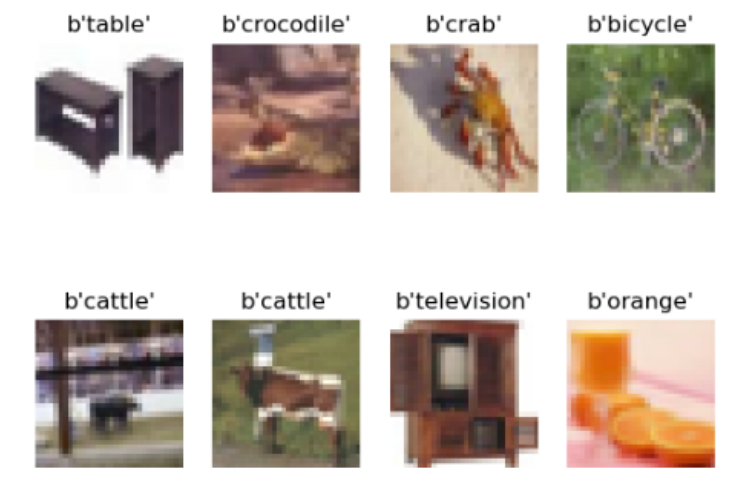
\includegraphics[width=\linewidth]{bench/img/cifar100.png}\\[3pt]
{\scriptsize CIFAR-100, 100 classes, 32$\times$32}
\end{center}
\end{minipage}

\begin{thebibliography}{10}
\beamertemplatearticlebibitems
\tiny
\bibitem{PruningBench} C. Li \emph{et al.}, A Comprehensive Study of Structural
Pruning for Vision Models (2025)
\end{thebibliography}

\end{frame}


% ------------------------------ SLIDE 7 ------------------------------
\begin{frame}
\frametitle{Latency of the pruned models}
\framesubtitle{Edge TPU speed-up versus parameter reduction, and INT8 model size}

\benchlegendfit{leg:benchspeedup}

\begin{center}
\makebox[\linewidth][c]{%
\begin{tikzpicture}
\begin{axis}[benchpanel, scale only axis, width=2.5cm, height=2.5cm, name=pVGG,
  title={VGG-19}, title style={font=\small, yshift=0.62cm},
  xlabel={Parameter reduction (\%)},
  ylabel={Edge TPU speed-up ($\times$)},
  xmin=0, xmax=90, xtick={0,30,60,90}, enlarge x limits=false]
\addplot[mark=none, domain=0:90, samples=2, dashed, black, thin] {1};
\benchseven{bench/data/sp_vgg19.csv}
\draw[red!70!black, dash dot, thick] ({axis cs:58.76,0}|-{rel axis cs:0,0}) -- ({axis cs:58.76,0}|-{rel axis cs:0,1});
\end{axis}
\begin{axis}[scale only axis, width=2.5cm, height=2.5cm,
  at=(pVGG.south west), anchor=south west,
  axis x line*=top, axis y line=none, ytick=\empty, ymin=0, ymax=1,
  xmin=1.93, xmax=19.30, x dir=reverse, enlarge x limits=false,
  xtick={2,6,10,14,18}, tick label style={font=\scriptsize},
  xlabel={INT8 size (MB)}, label style={font=\scriptsize}]
\end{axis}
\end{tikzpicture}\hspace{0.3cm}
\begin{tikzpicture}
\begin{axis}[benchpanel, scale only axis, width=2.5cm, height=2.5cm, name=pR18,
  title={ResNet-18}, title style={font=\small, yshift=0.62cm},
  xlabel={Parameter reduction (\%)},
  xmin=0, xmax=90, xtick={0,30,60,90}, enlarge x limits=false]
\addplot[mark=none, domain=0:90, samples=2, dashed, black, thin] {1};
\benchseven{bench/data/sp_resnet18.csv}
\draw[red!70!black, dash dot, thick] ({axis cs:26.29,0}|-{rel axis cs:0,0}) -- ({axis cs:26.29,0}|-{rel axis cs:0,1});
\end{axis}
\begin{axis}[scale only axis, width=2.5cm, height=2.5cm,
  at=(pR18.south west), anchor=south west,
  axis x line*=top, axis y line=none, ytick=\empty, ymin=0, ymax=1,
  xmin=1.08, xmax=10.84, x dir=reverse, enlarge x limits=false,
  xtick={2,4,6,8,10}, tick label style={font=\scriptsize},
  xlabel={INT8 size (MB)}, label style={font=\scriptsize}]
\end{axis}
\end{tikzpicture}\hspace{0.3cm}
\begin{tikzpicture}
\begin{axis}[benchpanel, scale only axis, width=2.5cm, height=2.5cm, name=pGLN,
  title={GoogLeNet}, title style={font=\small, yshift=0.62cm},
  xlabel={Parameter reduction (\%)},
  xmin=0, xmax=90, xtick={0,30,60,90}, enlarge x limits=false]
\addplot[mark=none, domain=0:90, samples=2, dashed, black, thin] {1};
\benchseven{bench/data/sp_googlenet.csv}
\end{axis}
\begin{axis}[scale only axis, width=2.5cm, height=2.5cm,
  at=(pGLN.south west), anchor=south west,
  axis x line*=top, axis y line=none, ytick=\empty, ymin=0, ymax=1,
  xmin=0.57, xmax=5.66, x dir=reverse, enlarge x limits=false,
  xtick={1,2,3,4,5}, tick label style={font=\scriptsize},
  xlabel={INT8 size (MB)}, label style={font=\scriptsize}]
\end{axis}
\end{tikzpicture}}

\vspace{3pt}
\ref{leg:benchspeedup}

\vspace{3pt}
{\small Red line: the rate at which the model first fits entirely on chip.
Note that each panel has its own vertical scale.}
\end{center}

\end{frame}


% ------------------------------ SLIDE 8 ------------------------------
\begin{frame}
\frametitle{Accuracy}
\framesubtitle{ResNet-18: accuracy right after pruning, and recovery fine-tuning}

\benchlegend{leg:benchacc}

\begin{center}
\makebox[\linewidth][c]{%
\begin{tikzpicture}
\begin{groupplot}[
  group style={group size=2 by 1, horizontal sep=1.5cm},
  benchpanel, scale only axis, width=3.1cm, height=3.1cm,
  title style={font=\small}]

\nextgroupplot[title={After pruning, before FT},
               xlabel={Pruning target (\%)}, ylabel={Top-1 val.\ acc.\ (\%)},
               xtick={10,30,50,70,90}]
\addplot[mark=none, domain=10:90, samples=2, dashed, black, thin] {76.890};
\benchseven{bench/data/pp_resnet18.csv}

\nextgroupplot[title={Recovery FT at 90\,\%},
               xlabel={Epoch}, ylabel={Top-1 val.\ acc.\ (\%)},
               xtick={0,50,100}]
\addplot[mark=none, domain=0:100, samples=2, dashed, black, thin, forget plot] {76.890};
\addplot[benchcurves, color=impmagnitudel1] table[x=epoch, y=magnitude_l1, col sep=comma] {bench/data/ft_resnet18_90.csv};
\addplot[benchcurves, color=impmagnitudel2] table[x=epoch, y=magnitude_l2, col sep=comma] {bench/data/ft_resnet18_90.csv};
\addplot[benchcurves, color=impbnscale]     table[x=epoch, y=bn_scale,     col sep=comma] {bench/data/ft_resnet18_90.csv};
\addplot[benchcurves, color=impfpgm]        table[x=epoch, y=fpgm,         col sep=comma] {bench/data/ft_resnet18_90.csv};
\addplot[benchcurves, color=imptaylor]      table[x=epoch, y=taylor,       col sep=comma] {bench/data/ft_resnet18_90.csv};
\addplot[benchcurves, color=impobdc]        table[x=epoch, y=obdc,         col sep=comma] {bench/data/ft_resnet18_90.csv};
\addplot[benchcurves, color=imprandom]      table[x=epoch, y=random,       col sep=comma] {bench/data/ft_resnet18_90.csv};

\end{groupplot}
\end{tikzpicture}}

\vspace{3pt}
\ref{leg:benchacc}

\vspace{3pt}
{\small Dashed line: unpruned baseline. Both indicators give the same ranking.}
\end{center}

\end{frame}


% ------------------------------ SLIDE 9 -----------------------------
\begin{frame}
\frametitle{Accuracy and latency disagree}
\framesubtitle{ResNet-50: the criterion that best preserves accuracy is the slowest}

\benchlegendfit{leg:benchboth}

\begin{center}
\makebox[\linewidth][c]{%
\begin{tikzpicture}
\begin{groupplot}[
  group style={group size=2 by 1, horizontal sep=1.5cm},
  benchpanel, scale only axis, width=3.1cm, height=3.1cm,
  title style={font=\small},
  xlabel={Parameter reduction (\%)}]

\nextgroupplot[title={Accuracy right after pruning},
               ylabel={Top-1 val.\ acc.\ (\%)}]
\addplot[mark=none, domain=10:90, samples=2, dashed, black, thin] {77.810};
\benchseven{bench/data/pp_resnet50.csv}

\nextgroupplot[title={Edge TPU speed-up}, ylabel={Speed-up ($\times$)}]
\addplot[mark=none, domain=0:90, samples=2, dashed, black, thin] {1};
\benchseven{bench/data/sp_resnet50.csv}
\draw[red!70!black, dash dot, thick] ({axis cs:65.90,0}|-{rel axis cs:0,0}) -- ({axis cs:65.90,0}|-{rel axis cs:0,1});

\end{groupplot}
\end{tikzpicture}}

\vspace{2pt}
\ref{leg:benchboth}

\vspace{2pt}
{\small At equal parameter reduction, two criteria do not produce the same
on-chip footprint: \emph{where} channels are removed matters.}
\end{center}

\end{frame}


% ------------------------------ SLIDE 10 -----------------------------
\begin{frame}
\frametitle{Real-time scheduling of multiple DNNs on a single TPU}
\framesubtitle{Illustrative use case}

\begin{minipage}{0.64\textwidth}
{\small
\begin{itemize}\setlength{\itemsep}{3pt}
  \item[{\color{blue!80!black}$\bullet$}] Single TPU
  \item[{\color{blue!80!black}$\bullet$}] Many DNNs executed at different rates
  \item[{\color{blue!80!black}$\bullet$}] \emph{Earliest Deadline First (EDF)}
  \item[{\color{blue!80!black}$\bullet$}] Non-preemptive avoids weight reloading
  \item[{\color{blue!80!black}$\bullet$}] Sporadic tasks (\emph{i.e.,} event-triggered)
\end{itemize}}

\vspace{0.25cm}

\setlength{\tabcolsep}{4pt}
\renewcommand{\arraystretch}{0.95}
{\tiny
\begin{tabular}{llrrr}
\toprule
Function & Model & $T$ (ms) & $C$ (ms) & $C/T$ \\
\midrule
Nozzle trigger    & ResNet-18    &  20 & 11.4 & 0.57 \\
Crop growth stage & MobileNetV2  &  33 &  1.2 & 0.04 \\
Weed species      & ResNet-50    & 100 & 50.9 & 0.51 \\
Ground cover      & VGG-19       & 200 & 39.3 & 0.20 \\
\midrule
\multicolumn{4}{r}{Total utilization} & \textbf{\color{red!80!black}1.32} \\
\bottomrule
\end{tabular}}

\vspace{0.2cm}
{\small \color{red!80!black}$U > 1$ : the task set is \textbf{infeasible}.}
\end{minipage}\hfill
\begin{minipage}{0.32\textwidth}
\begin{center}
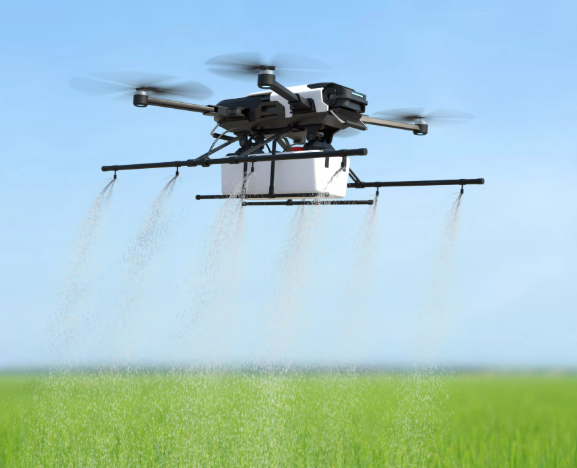
\includegraphics[width=\linewidth]{bench/img/drone_rampe_de_buses.png}\\[5pt]
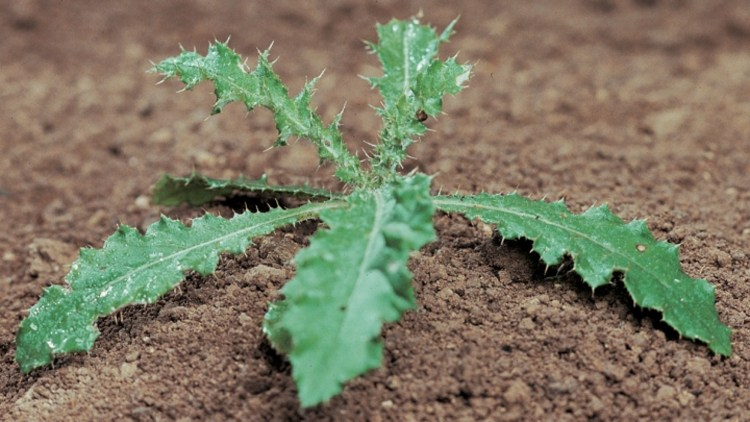
\includegraphics[width=\linewidth]{bench/img/adventice.jpg}
\end{center}
\end{minipage}

\vspace{0.2cm}

\begin{thebibliography}{10}
\beamertemplatearticlebibitems
\tiny
\bibitem{Buttazzo} G. Buttazzo, Can We Trust AI-Powered Real-Time Embedded
Systems? NG-RES (2022)
\end{thebibliography}

\end{frame}

%  Prerequis (deja dans le preambule) : pgfplots + groupplots, graphicx,
%  booktabs, tikz, xcolor.
%  Donnees : bench/data/*.csv       Images : bench/img/*
%  Les figures sont en pgfplots, meme rendu que les figures de l'article.
% =====================================================================

% --- palette des criteres d'importance (identique a celle de l'article) ---
\definecolor{impmagnitudel1}{HTML}{1F77B4}
\definecolor{impmagnitudel2}{HTML}{AEC7E8}
\definecolor{impbnscale}{HTML}{FF7F0E}
\definecolor{impfpgm}{HTML}{2CA02C}
\definecolor{imptaylor}{HTML}{D62728}
\definecolor{impobdc}{HTML}{9467BD}
\definecolor{imprandom}{HTML}{7F7F7F}

% --- style commun a tous les panneaux ---
\pgfplotsset{
  benchpanel/.style={
    grid=both, grid style={dashed,gray!30},
    tick label style={font=\scriptsize},
    label style={font=\scriptsize},
    title style={font=\small},
  },
  benchcurves/.style={mark=none, line width=1.0pt, unbounded coords=jump},
}

% --- legende partagee (7 criteres), construite une fois par frame ---
\newcommand{\benchlegendcore}[2]{%
\begin{tikzpicture}
\begin{axis}[hide axis, scale only axis, width=1pt, height=1pt,
  xmin=0, xmax=1, ymin=0, ymax=1,
  legend columns=4, legend to name=#1,
  legend style={draw=gray!50, font=\scriptsize, /tikz/every even column/.append style={column sep=6pt}}]
\addplot[draw=none, forget plot] coordinates {(0,0)};
\addlegendimage{color=impmagnitudel1, line width=1.0pt}\addlegendentry{Magnitude L1}
\addlegendimage{color=impmagnitudel2, line width=1.0pt}\addlegendentry{Magnitude L2}
\addlegendimage{color=impbnscale, line width=1.0pt}\addlegendentry{BN-Scale}
\addlegendimage{color=impfpgm, line width=1.0pt}\addlegendentry{FPGM}
\addlegendimage{color=imptaylor, line width=1.0pt}\addlegendentry{Taylor}
\addlegendimage{color=impobdc, line width=1.0pt}\addlegendentry{OBD-C}
\addlegendimage{color=imprandom, line width=1.0pt}\addlegendentry{Random}
#2
\end{axis}
\end{tikzpicture}}
\newcommand{\benchlegend}[1]{\benchlegendcore{#1}{}}
\newcommand{\benchlegendfit}[1]{\benchlegendcore{#1}{%
\addlegendimage{color=red!70!black, dash dot, line width=1.0pt}\addlegendentry{Fits 8\,MB SRAM}}}

% --- les 7 courbes d'un fichier CSV (colonnes <crit>_x / <crit>_y) ---
\newcommand{\benchseven}[1]{%
\addplot[benchcurves, color=impmagnitudel1] table[x=magl1_x,   y=magl1_y,   col sep=comma] {#1};
\addplot[benchcurves, color=impmagnitudel2] table[x=magl2_x,   y=magl2_y,   col sep=comma] {#1};
\addplot[benchcurves, color=impbnscale]     table[x=bnscale_x, y=bnscale_y, col sep=comma] {#1};
\addplot[benchcurves, color=impfpgm]        table[x=fpgm_x,    y=fpgm_y,    col sep=comma] {#1};
\addplot[benchcurves, color=imptaylor]      table[x=taylor_x,  y=taylor_y,  col sep=comma] {#1};
\addplot[benchcurves, color=impobdc]        table[x=obdc_x,    y=obdc_y,    col sep=comma] {#1};
\addplot[benchcurves, color=imprandom]      table[x=random_x,  y=random_y,  col sep=comma] {#1};}


% =====================================================================
\section{Measurement study}
% =====================================================================

% ------------------------------ SLIDE 6 ------------------------------
\begin{frame}
\frametitle{Benchmark on the Coral USB Edge TPU}

\vspace{0.15cm}

\begin{minipage}[t]{0.48\textwidth}\vspace{0pt}
{\scriptsize
\setlength{\tabcolsep}{4pt}
\begin{tabularx}{\linewidth}{@{}l >{\raggedright\arraybackslash}X@{}}
\toprule
\multicolumn{2}{c}{\textbf{7 architectures, by topology}}\\
\midrule
Sequential        & VGG-19 \\
Residual          & ResNet-18, ResNet-50, WRN-28-10 \\
Inverted residual & MobileNetV2 \\
Concatenation     & GoogLeNet, SqueezeNet 1.1 \\
\bottomrule
\end{tabularx}}
\end{minipage}\hfill
\begin{minipage}[t]{0.48\textwidth}\vspace{0pt}
{\scriptsize
\setlength{\tabcolsep}{4pt}
\begin{tabularx}{\linewidth}{@{}l >{\raggedright\arraybackslash}X@{}}
\toprule
\multicolumn{2}{c}{\textbf{7 criteria, by information used}}\\
\midrule
Data-free \,{\tiny(weights)}   & Magnitude L1, L2, FPGM \\
Sparsity learning              & BN-Scale \\
Data-driven \,{\tiny(fwd+bwd)} & Taylor, OBD-C \\
Control                        & Random \\
\bottomrule
\end{tabularx}}
\end{minipage}

\vspace{0.4cm}

\begin{minipage}[c]{0.58\textwidth}
{\small
\begin{itemize}\setlength{\itemsep}{8pt}
  \item[{\color{blue!80!black}$\bullet$}]
    \textbf{9 compression rates}\\
    10\,\% to 90\,\% of parameters removed, in steps of 10.
  \item[{\color{blue!80!black}$\bullet$}]
    \textbf{PruningBench protocol}~[1]\\
    Unchanged: 400 iterative steps, global ranking, 100 recovery epochs.\\
    {\scriptsize 404 of the 441 combinations reached the accelerator.}
\end{itemize}}
\end{minipage}\hfill
\begin{minipage}[c]{0.38\textwidth}
\begin{center}
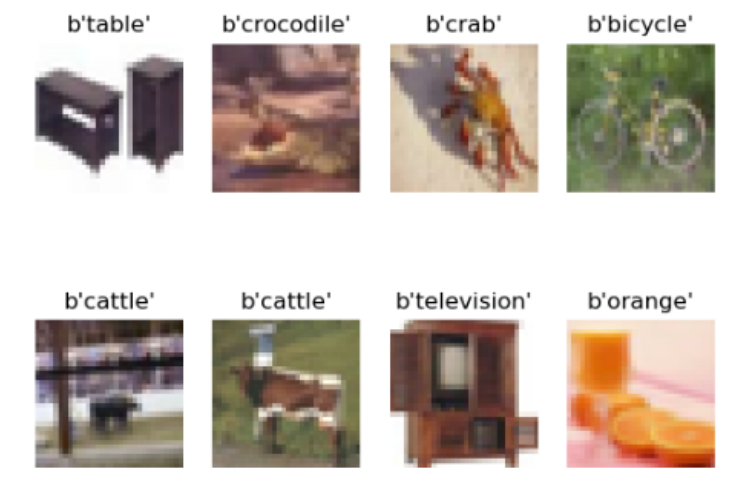
\includegraphics[width=\linewidth]{bench/img/cifar100.png}\\[3pt]
{\scriptsize CIFAR-100, 100 classes, 32$\times$32}
\end{center}
\end{minipage}

\begin{thebibliography}{10}
\beamertemplatearticlebibitems
\tiny
\bibitem{PruningBench} C. Li \emph{et al.}, A Comprehensive Study of Structural
Pruning for Vision Models (2025)
\end{thebibliography}

\end{frame}


% ------------------------------ SLIDE 7 ------------------------------
\begin{frame}
\frametitle{Latency of the pruned models}
\framesubtitle{Edge TPU speed-up versus parameter reduction, and INT8 model size}

\benchlegendfit{leg:benchspeedup}

\begin{center}
\makebox[\linewidth][c]{%
\begin{tikzpicture}
\begin{axis}[benchpanel, scale only axis, width=2.5cm, height=2.5cm, name=pVGG,
  title={VGG-19}, title style={font=\small, yshift=0.62cm},
  xlabel={Parameter reduction (\%)},
  ylabel={Edge TPU speed-up ($\times$)},
  xmin=0, xmax=90, xtick={0,30,60,90}, enlarge x limits=false]
\addplot[mark=none, domain=0:90, samples=2, dashed, black, thin] {1};
\benchseven{bench/data/sp_vgg19.csv}
\draw[red!70!black, dash dot, thick] ({axis cs:58.76,0}|-{rel axis cs:0,0}) -- ({axis cs:58.76,0}|-{rel axis cs:0,1});
\end{axis}
\begin{axis}[scale only axis, width=2.5cm, height=2.5cm,
  at=(pVGG.south west), anchor=south west,
  axis x line*=top, axis y line=none, ytick=\empty, ymin=0, ymax=1,
  xmin=1.93, xmax=19.30, x dir=reverse, enlarge x limits=false,
  xtick={2,6,10,14,18}, tick label style={font=\scriptsize},
  xlabel={INT8 size (MB)}, label style={font=\scriptsize}]
\end{axis}
\end{tikzpicture}\hspace{0.3cm}
\begin{tikzpicture}
\begin{axis}[benchpanel, scale only axis, width=2.5cm, height=2.5cm, name=pR18,
  title={ResNet-18}, title style={font=\small, yshift=0.62cm},
  xlabel={Parameter reduction (\%)},
  xmin=0, xmax=90, xtick={0,30,60,90}, enlarge x limits=false]
\addplot[mark=none, domain=0:90, samples=2, dashed, black, thin] {1};
\benchseven{bench/data/sp_resnet18.csv}
\draw[red!70!black, dash dot, thick] ({axis cs:26.29,0}|-{rel axis cs:0,0}) -- ({axis cs:26.29,0}|-{rel axis cs:0,1});
\end{axis}
\begin{axis}[scale only axis, width=2.5cm, height=2.5cm,
  at=(pR18.south west), anchor=south west,
  axis x line*=top, axis y line=none, ytick=\empty, ymin=0, ymax=1,
  xmin=1.08, xmax=10.84, x dir=reverse, enlarge x limits=false,
  xtick={2,4,6,8,10}, tick label style={font=\scriptsize},
  xlabel={INT8 size (MB)}, label style={font=\scriptsize}]
\end{axis}
\end{tikzpicture}\hspace{0.3cm}
\begin{tikzpicture}
\begin{axis}[benchpanel, scale only axis, width=2.5cm, height=2.5cm, name=pGLN,
  title={GoogLeNet}, title style={font=\small, yshift=0.62cm},
  xlabel={Parameter reduction (\%)},
  xmin=0, xmax=90, xtick={0,30,60,90}, enlarge x limits=false]
\addplot[mark=none, domain=0:90, samples=2, dashed, black, thin] {1};
\benchseven{bench/data/sp_googlenet.csv}
\end{axis}
\begin{axis}[scale only axis, width=2.5cm, height=2.5cm,
  at=(pGLN.south west), anchor=south west,
  axis x line*=top, axis y line=none, ytick=\empty, ymin=0, ymax=1,
  xmin=0.57, xmax=5.66, x dir=reverse, enlarge x limits=false,
  xtick={1,2,3,4,5}, tick label style={font=\scriptsize},
  xlabel={INT8 size (MB)}, label style={font=\scriptsize}]
\end{axis}
\end{tikzpicture}}

\vspace{3pt}
\ref{leg:benchspeedup}

\vspace{3pt}
{\small Red line: the rate at which the model first fits entirely on chip.
Note that each panel has its own vertical scale.}
\end{center}

\end{frame}


% ------------------------------ SLIDE 8 ------------------------------
\begin{frame}
\frametitle{Accuracy}
\framesubtitle{ResNet-18: accuracy right after pruning, and recovery fine-tuning}

\benchlegend{leg:benchacc}

\begin{center}
\makebox[\linewidth][c]{%
\begin{tikzpicture}
\begin{groupplot}[
  group style={group size=2 by 1, horizontal sep=1.5cm},
  benchpanel, scale only axis, width=3.1cm, height=3.1cm,
  title style={font=\small}]

\nextgroupplot[title={After pruning, before FT},
               xlabel={Pruning target (\%)}, ylabel={Top-1 val.\ acc.\ (\%)},
               xtick={10,30,50,70,90}]
\addplot[mark=none, domain=10:90, samples=2, dashed, black, thin] {76.890};
\benchseven{bench/data/pp_resnet18.csv}

\nextgroupplot[title={Recovery FT at 90\,\%},
               xlabel={Epoch}, ylabel={Top-1 val.\ acc.\ (\%)},
               xtick={0,50,100}]
\addplot[mark=none, domain=0:100, samples=2, dashed, black, thin, forget plot] {76.890};
\addplot[benchcurves, color=impmagnitudel1] table[x=epoch, y=magnitude_l1, col sep=comma] {bench/data/ft_resnet18_90.csv};
\addplot[benchcurves, color=impmagnitudel2] table[x=epoch, y=magnitude_l2, col sep=comma] {bench/data/ft_resnet18_90.csv};
\addplot[benchcurves, color=impbnscale]     table[x=epoch, y=bn_scale,     col sep=comma] {bench/data/ft_resnet18_90.csv};
\addplot[benchcurves, color=impfpgm]        table[x=epoch, y=fpgm,         col sep=comma] {bench/data/ft_resnet18_90.csv};
\addplot[benchcurves, color=imptaylor]      table[x=epoch, y=taylor,       col sep=comma] {bench/data/ft_resnet18_90.csv};
\addplot[benchcurves, color=impobdc]        table[x=epoch, y=obdc,         col sep=comma] {bench/data/ft_resnet18_90.csv};
\addplot[benchcurves, color=imprandom]      table[x=epoch, y=random,       col sep=comma] {bench/data/ft_resnet18_90.csv};

\end{groupplot}
\end{tikzpicture}}

\vspace{3pt}
\ref{leg:benchacc}

\vspace{3pt}
{\small Dashed line: unpruned baseline. Both indicators give the same ranking.}
\end{center}

\end{frame}


% ------------------------------ SLIDE 9 -----------------------------
\begin{frame}
\frametitle{Accuracy and latency disagree}
\framesubtitle{ResNet-50: the criterion that best preserves accuracy is the slowest}

\benchlegendfit{leg:benchboth}

\begin{center}
\makebox[\linewidth][c]{%
\begin{tikzpicture}
\begin{groupplot}[
  group style={group size=2 by 1, horizontal sep=1.5cm},
  benchpanel, scale only axis, width=3.1cm, height=3.1cm,
  title style={font=\small},
  xlabel={Parameter reduction (\%)}]

\nextgroupplot[title={Accuracy right after pruning},
               ylabel={Top-1 val.\ acc.\ (\%)}]
\addplot[mark=none, domain=10:90, samples=2, dashed, black, thin] {77.810};
\benchseven{bench/data/pp_resnet50.csv}

\nextgroupplot[title={Edge TPU speed-up}, ylabel={Speed-up ($\times$)}]
\addplot[mark=none, domain=0:90, samples=2, dashed, black, thin] {1};
\benchseven{bench/data/sp_resnet50.csv}
\draw[red!70!black, dash dot, thick] ({axis cs:65.90,0}|-{rel axis cs:0,0}) -- ({axis cs:65.90,0}|-{rel axis cs:0,1});

\end{groupplot}
\end{tikzpicture}}

\vspace{2pt}
\ref{leg:benchboth}

\vspace{2pt}
{\small At equal parameter reduction, two criteria do not produce the same
on-chip footprint: \emph{where} channels are removed matters.}
\end{center}

\end{frame}


% ------------------------------ SLIDE 10 -----------------------------
\begin{frame}
\frametitle{Real-time scheduling of multiple DNNs on a single TPU}
\framesubtitle{Illustrative use case}

\begin{minipage}{0.64\textwidth}
{\small
\begin{itemize}\setlength{\itemsep}{3pt}
  \item[{\color{blue!80!black}$\bullet$}] Single TPU
  \item[{\color{blue!80!black}$\bullet$}] Many DNNs executed at different rates
  \item[{\color{blue!80!black}$\bullet$}] \emph{Earliest Deadline First (EDF)}
  \item[{\color{blue!80!black}$\bullet$}] Non-preemptive avoids weight reloading
  \item[{\color{blue!80!black}$\bullet$}] Sporadic tasks (\emph{i.e.,} event-triggered)
\end{itemize}}

\vspace{0.25cm}

\setlength{\tabcolsep}{4pt}
\renewcommand{\arraystretch}{0.95}
{\tiny
\begin{tabular}{llrrr}
\toprule
Function & Model & $T$ (ms) & $C$ (ms) & $C/T$ \\
\midrule
Nozzle trigger    & ResNet-18    &  20 & 11.4 & 0.57 \\
Crop growth stage & MobileNetV2  &  33 &  1.2 & 0.04 \\
Weed species      & ResNet-50    & 100 & 50.9 & 0.51 \\
Ground cover      & VGG-19       & 200 & 39.3 & 0.20 \\
\midrule
\multicolumn{4}{r}{Total utilization} & \textbf{\color{red!80!black}1.32} \\
\bottomrule
\end{tabular}}

\vspace{0.2cm}
{\small \color{red!80!black}$U > 1$ : the task set is \textbf{infeasible}.}
\end{minipage}\hfill
\begin{minipage}{0.32\textwidth}
\begin{center}
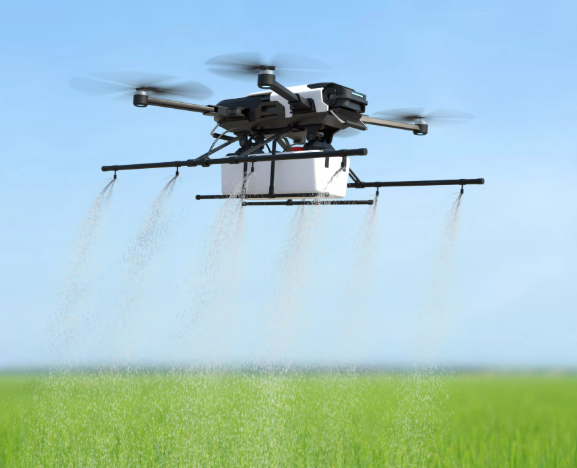
\includegraphics[width=\linewidth]{bench/img/drone_rampe_de_buses.png}\\[5pt]
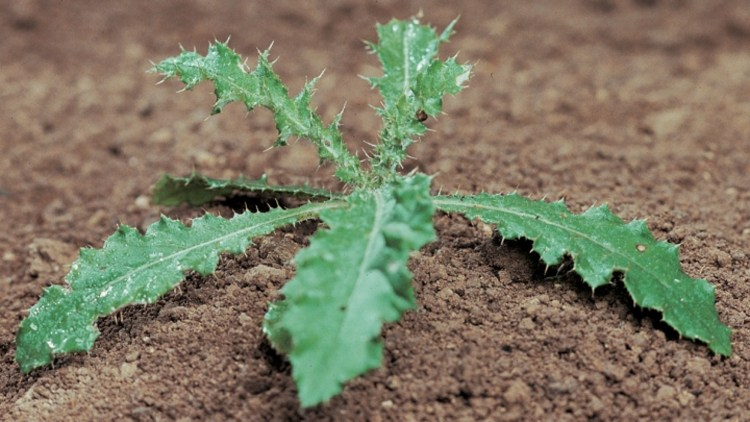
\includegraphics[width=\linewidth]{bench/img/adventice.jpg}
\end{center}
\end{minipage}

\vspace{0.2cm}

\begin{thebibliography}{10}
\beamertemplatearticlebibitems
\tiny
\bibitem{Buttazzo} G. Buttazzo, Can We Trust AI-Powered Real-Time Embedded
Systems? NG-RES (2022)
\end{thebibliography}

\end{frame}

%  Prerequis (deja dans le preambule) : pgfplots + groupplots, graphicx,
%  booktabs, tikz, xcolor.
%  Donnees : bench/data/*.csv       Images : bench/img/*
%  Les figures sont en pgfplots, meme rendu que les figures de l'article.
% =====================================================================

% --- palette des criteres d'importance (identique a celle de l'article) ---
\definecolor{impmagnitudel1}{HTML}{1F77B4}
\definecolor{impmagnitudel2}{HTML}{AEC7E8}
\definecolor{impbnscale}{HTML}{FF7F0E}
\definecolor{impfpgm}{HTML}{2CA02C}
\definecolor{imptaylor}{HTML}{D62728}
\definecolor{impobdc}{HTML}{9467BD}
\definecolor{imprandom}{HTML}{7F7F7F}

% --- style commun a tous les panneaux ---
\pgfplotsset{
  benchpanel/.style={
    grid=both, grid style={dashed,gray!30},
    tick label style={font=\scriptsize},
    label style={font=\scriptsize},
    title style={font=\small},
  },
  benchcurves/.style={mark=none, line width=1.0pt, unbounded coords=jump},
}

% --- legende partagee (7 criteres), construite une fois par frame ---
\newcommand{\benchlegendcore}[2]{%
\begin{tikzpicture}
\begin{axis}[hide axis, scale only axis, width=1pt, height=1pt,
  xmin=0, xmax=1, ymin=0, ymax=1,
  legend columns=4, legend to name=#1,
  legend style={draw=gray!50, font=\scriptsize, /tikz/every even column/.append style={column sep=6pt}}]
\addplot[draw=none, forget plot] coordinates {(0,0)};
\addlegendimage{color=impmagnitudel1, line width=1.0pt}\addlegendentry{Magnitude L1}
\addlegendimage{color=impmagnitudel2, line width=1.0pt}\addlegendentry{Magnitude L2}
\addlegendimage{color=impbnscale, line width=1.0pt}\addlegendentry{BN-Scale}
\addlegendimage{color=impfpgm, line width=1.0pt}\addlegendentry{FPGM}
\addlegendimage{color=imptaylor, line width=1.0pt}\addlegendentry{Taylor}
\addlegendimage{color=impobdc, line width=1.0pt}\addlegendentry{OBD-C}
\addlegendimage{color=imprandom, line width=1.0pt}\addlegendentry{Random}
#2
\end{axis}
\end{tikzpicture}}
\newcommand{\benchlegend}[1]{\benchlegendcore{#1}{}}
\newcommand{\benchlegendfit}[1]{\benchlegendcore{#1}{%
\addlegendimage{color=red!70!black, dash dot, line width=1.0pt}\addlegendentry{Fits 8\,MB SRAM}}}

% --- les 7 courbes d'un fichier CSV (colonnes <crit>_x / <crit>_y) ---
\newcommand{\benchseven}[1]{%
\addplot[benchcurves, color=impmagnitudel1] table[x=magl1_x,   y=magl1_y,   col sep=comma] {#1};
\addplot[benchcurves, color=impmagnitudel2] table[x=magl2_x,   y=magl2_y,   col sep=comma] {#1};
\addplot[benchcurves, color=impbnscale]     table[x=bnscale_x, y=bnscale_y, col sep=comma] {#1};
\addplot[benchcurves, color=impfpgm]        table[x=fpgm_x,    y=fpgm_y,    col sep=comma] {#1};
\addplot[benchcurves, color=imptaylor]      table[x=taylor_x,  y=taylor_y,  col sep=comma] {#1};
\addplot[benchcurves, color=impobdc]        table[x=obdc_x,    y=obdc_y,    col sep=comma] {#1};
\addplot[benchcurves, color=imprandom]      table[x=random_x,  y=random_y,  col sep=comma] {#1};}


% =====================================================================
\section{Measurement study}
% =====================================================================

% ------------------------------ SLIDE 6 ------------------------------
\begin{frame}
\frametitle{Benchmark on the Coral USB Edge TPU}

\vspace{0.15cm}

\begin{minipage}[t]{0.48\textwidth}\vspace{0pt}
{\scriptsize
\setlength{\tabcolsep}{4pt}
\begin{tabularx}{\linewidth}{@{}l >{\raggedright\arraybackslash}X@{}}
\toprule
\multicolumn{2}{c}{\textbf{7 architectures, by topology}}\\
\midrule
Sequential        & VGG-19 \\
Residual          & ResNet-18, ResNet-50, WRN-28-10 \\
Inverted residual & MobileNetV2 \\
Concatenation     & GoogLeNet, SqueezeNet 1.1 \\
\bottomrule
\end{tabularx}}
\end{minipage}\hfill
\begin{minipage}[t]{0.48\textwidth}\vspace{0pt}
{\scriptsize
\setlength{\tabcolsep}{4pt}
\begin{tabularx}{\linewidth}{@{}l >{\raggedright\arraybackslash}X@{}}
\toprule
\multicolumn{2}{c}{\textbf{7 criteria, by information used}}\\
\midrule
Data-free \,{\tiny(weights)}   & Magnitude L1, L2, FPGM \\
Sparsity learning              & BN-Scale \\
Data-driven \,{\tiny(fwd+bwd)} & Taylor, OBD-C \\
Control                        & Random \\
\bottomrule
\end{tabularx}}
\end{minipage}

\vspace{0.4cm}

\begin{minipage}[c]{0.58\textwidth}
{\small
\begin{itemize}\setlength{\itemsep}{8pt}
  \item[{\color{blue!80!black}$\bullet$}]
    \textbf{9 compression rates}\\
    10\,\% to 90\,\% of parameters removed, in steps of 10.
  \item[{\color{blue!80!black}$\bullet$}]
    \textbf{PruningBench protocol}~[1]\\
    Unchanged: 400 iterative steps, global ranking, 100 recovery epochs.\\
    {\scriptsize 404 of the 441 combinations reached the accelerator.}
\end{itemize}}
\end{minipage}\hfill
\begin{minipage}[c]{0.38\textwidth}
\begin{center}
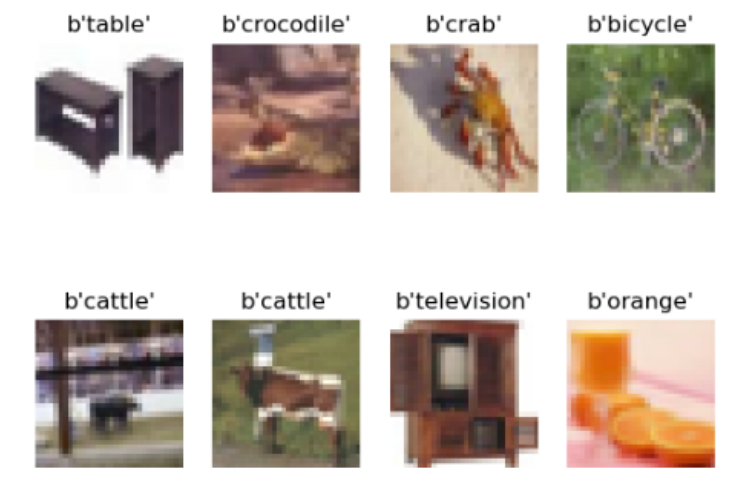
\includegraphics[width=\linewidth]{bench/img/cifar100.png}\\[3pt]
{\scriptsize CIFAR-100, 100 classes, 32$\times$32}
\end{center}
\end{minipage}

\begin{thebibliography}{10}
\beamertemplatearticlebibitems
\tiny
\bibitem{PruningBench} C. Li \emph{et al.}, A Comprehensive Study of Structural
Pruning for Vision Models (2025)
\end{thebibliography}

\end{frame}


% ------------------------------ SLIDE 7 ------------------------------
\begin{frame}
\frametitle{Latency of the pruned models}
\framesubtitle{Edge TPU speed-up versus parameter reduction, and INT8 model size}

\benchlegendfit{leg:benchspeedup}

\begin{center}
\makebox[\linewidth][c]{%
\begin{tikzpicture}
\begin{axis}[benchpanel, scale only axis, width=2.5cm, height=2.5cm, name=pVGG,
  title={VGG-19}, title style={font=\small, yshift=0.62cm},
  xlabel={Parameter reduction (\%)},
  ylabel={Edge TPU speed-up ($\times$)},
  xmin=0, xmax=90, xtick={0,30,60,90}, enlarge x limits=false]
\addplot[mark=none, domain=0:90, samples=2, dashed, black, thin] {1};
\benchseven{bench/data/sp_vgg19.csv}
\draw[red!70!black, dash dot, thick] ({axis cs:58.76,0}|-{rel axis cs:0,0}) -- ({axis cs:58.76,0}|-{rel axis cs:0,1});
\end{axis}
\begin{axis}[scale only axis, width=2.5cm, height=2.5cm,
  at=(pVGG.south west), anchor=south west,
  axis x line*=top, axis y line=none, ytick=\empty, ymin=0, ymax=1,
  xmin=1.93, xmax=19.30, x dir=reverse, enlarge x limits=false,
  xtick={2,6,10,14,18}, tick label style={font=\scriptsize},
  xlabel={INT8 size (MB)}, label style={font=\scriptsize}]
\end{axis}
\end{tikzpicture}\hspace{0.3cm}
\begin{tikzpicture}
\begin{axis}[benchpanel, scale only axis, width=2.5cm, height=2.5cm, name=pR18,
  title={ResNet-18}, title style={font=\small, yshift=0.62cm},
  xlabel={Parameter reduction (\%)},
  xmin=0, xmax=90, xtick={0,30,60,90}, enlarge x limits=false]
\addplot[mark=none, domain=0:90, samples=2, dashed, black, thin] {1};
\benchseven{bench/data/sp_resnet18.csv}
\draw[red!70!black, dash dot, thick] ({axis cs:26.29,0}|-{rel axis cs:0,0}) -- ({axis cs:26.29,0}|-{rel axis cs:0,1});
\end{axis}
\begin{axis}[scale only axis, width=2.5cm, height=2.5cm,
  at=(pR18.south west), anchor=south west,
  axis x line*=top, axis y line=none, ytick=\empty, ymin=0, ymax=1,
  xmin=1.08, xmax=10.84, x dir=reverse, enlarge x limits=false,
  xtick={2,4,6,8,10}, tick label style={font=\scriptsize},
  xlabel={INT8 size (MB)}, label style={font=\scriptsize}]
\end{axis}
\end{tikzpicture}\hspace{0.3cm}
\begin{tikzpicture}
\begin{axis}[benchpanel, scale only axis, width=2.5cm, height=2.5cm, name=pGLN,
  title={GoogLeNet}, title style={font=\small, yshift=0.62cm},
  xlabel={Parameter reduction (\%)},
  xmin=0, xmax=90, xtick={0,30,60,90}, enlarge x limits=false]
\addplot[mark=none, domain=0:90, samples=2, dashed, black, thin] {1};
\benchseven{bench/data/sp_googlenet.csv}
\end{axis}
\begin{axis}[scale only axis, width=2.5cm, height=2.5cm,
  at=(pGLN.south west), anchor=south west,
  axis x line*=top, axis y line=none, ytick=\empty, ymin=0, ymax=1,
  xmin=0.57, xmax=5.66, x dir=reverse, enlarge x limits=false,
  xtick={1,2,3,4,5}, tick label style={font=\scriptsize},
  xlabel={INT8 size (MB)}, label style={font=\scriptsize}]
\end{axis}
\end{tikzpicture}}

\vspace{3pt}
\ref{leg:benchspeedup}

\vspace{3pt}
{\small Red line: the rate at which the model first fits entirely on chip.
Note that each panel has its own vertical scale.}
\end{center}

\end{frame}


% ------------------------------ SLIDE 8 ------------------------------
\begin{frame}
\frametitle{Accuracy}
\framesubtitle{ResNet-18: accuracy right after pruning, and recovery fine-tuning}

\benchlegend{leg:benchacc}

\begin{center}
\makebox[\linewidth][c]{%
\begin{tikzpicture}
\begin{groupplot}[
  group style={group size=2 by 1, horizontal sep=1.5cm},
  benchpanel, scale only axis, width=3.1cm, height=3.1cm,
  title style={font=\small}]

\nextgroupplot[title={After pruning, before FT},
               xlabel={Pruning target (\%)}, ylabel={Top-1 val.\ acc.\ (\%)},
               xtick={10,30,50,70,90}]
\addplot[mark=none, domain=10:90, samples=2, dashed, black, thin] {76.890};
\benchseven{bench/data/pp_resnet18.csv}

\nextgroupplot[title={Recovery FT at 90\,\%},
               xlabel={Epoch}, ylabel={Top-1 val.\ acc.\ (\%)},
               xtick={0,50,100}]
\addplot[mark=none, domain=0:100, samples=2, dashed, black, thin, forget plot] {76.890};
\addplot[benchcurves, color=impmagnitudel1] table[x=epoch, y=magnitude_l1, col sep=comma] {bench/data/ft_resnet18_90.csv};
\addplot[benchcurves, color=impmagnitudel2] table[x=epoch, y=magnitude_l2, col sep=comma] {bench/data/ft_resnet18_90.csv};
\addplot[benchcurves, color=impbnscale]     table[x=epoch, y=bn_scale,     col sep=comma] {bench/data/ft_resnet18_90.csv};
\addplot[benchcurves, color=impfpgm]        table[x=epoch, y=fpgm,         col sep=comma] {bench/data/ft_resnet18_90.csv};
\addplot[benchcurves, color=imptaylor]      table[x=epoch, y=taylor,       col sep=comma] {bench/data/ft_resnet18_90.csv};
\addplot[benchcurves, color=impobdc]        table[x=epoch, y=obdc,         col sep=comma] {bench/data/ft_resnet18_90.csv};
\addplot[benchcurves, color=imprandom]      table[x=epoch, y=random,       col sep=comma] {bench/data/ft_resnet18_90.csv};

\end{groupplot}
\end{tikzpicture}}

\vspace{3pt}
\ref{leg:benchacc}

\vspace{3pt}
{\small Dashed line: unpruned baseline. Both indicators give the same ranking.}
\end{center}

\end{frame}


% ------------------------------ SLIDE 9 -----------------------------
\begin{frame}
\frametitle{Accuracy and latency disagree}
\framesubtitle{ResNet-50: the criterion that best preserves accuracy is the slowest}

\benchlegendfit{leg:benchboth}

\begin{center}
\makebox[\linewidth][c]{%
\begin{tikzpicture}
\begin{groupplot}[
  group style={group size=2 by 1, horizontal sep=1.5cm},
  benchpanel, scale only axis, width=3.1cm, height=3.1cm,
  title style={font=\small},
  xlabel={Parameter reduction (\%)}]

\nextgroupplot[title={Accuracy right after pruning},
               ylabel={Top-1 val.\ acc.\ (\%)}]
\addplot[mark=none, domain=10:90, samples=2, dashed, black, thin] {77.810};
\benchseven{bench/data/pp_resnet50.csv}

\nextgroupplot[title={Edge TPU speed-up}, ylabel={Speed-up ($\times$)}]
\addplot[mark=none, domain=0:90, samples=2, dashed, black, thin] {1};
\benchseven{bench/data/sp_resnet50.csv}
\draw[red!70!black, dash dot, thick] ({axis cs:65.90,0}|-{rel axis cs:0,0}) -- ({axis cs:65.90,0}|-{rel axis cs:0,1});

\end{groupplot}
\end{tikzpicture}}

\vspace{2pt}
\ref{leg:benchboth}

\vspace{2pt}
{\small At equal parameter reduction, two criteria do not produce the same
on-chip footprint: \emph{where} channels are removed matters.}
\end{center}

\end{frame}


% ------------------------------ SLIDE 10 -----------------------------
\begin{frame}
\frametitle{Real-time scheduling of multiple DNNs on a single TPU}
\framesubtitle{Illustrative use case}

\begin{minipage}{0.64\textwidth}
{\small
\begin{itemize}\setlength{\itemsep}{3pt}
  \item[{\color{blue!80!black}$\bullet$}] Single TPU
  \item[{\color{blue!80!black}$\bullet$}] Many DNNs executed at different rates
  \item[{\color{blue!80!black}$\bullet$}] \emph{Earliest Deadline First (EDF)}
  \item[{\color{blue!80!black}$\bullet$}] Non-preemptive avoids weight reloading
  \item[{\color{blue!80!black}$\bullet$}] Sporadic tasks (\emph{i.e.,} event-triggered)
\end{itemize}}

\vspace{0.25cm}

\setlength{\tabcolsep}{4pt}
\renewcommand{\arraystretch}{0.95}
{\tiny
\begin{tabular}{llrrr}
\toprule
Function & Model & $T$ (ms) & $C$ (ms) & $C/T$ \\
\midrule
Nozzle trigger    & ResNet-18    &  20 & 11.4 & 0.57 \\
Crop growth stage & MobileNetV2  &  33 &  1.2 & 0.04 \\
Weed species      & ResNet-50    & 100 & 50.9 & 0.51 \\
Ground cover      & VGG-19       & 200 & 39.3 & 0.20 \\
\midrule
\multicolumn{4}{r}{Total utilization} & \textbf{\color{red!80!black}1.32} \\
\bottomrule
\end{tabular}}

\vspace{0.2cm}
{\small \color{red!80!black}$U > 1$ : the task set is \textbf{infeasible}.}
\end{minipage}\hfill
\begin{minipage}{0.32\textwidth}
\begin{center}
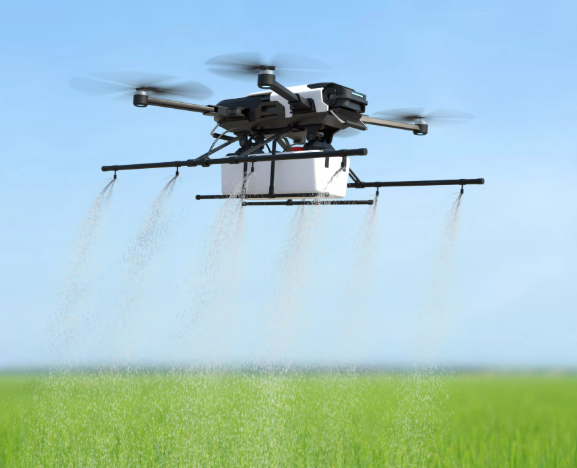
\includegraphics[width=\linewidth]{bench/img/drone_rampe_de_buses.png}\\[5pt]
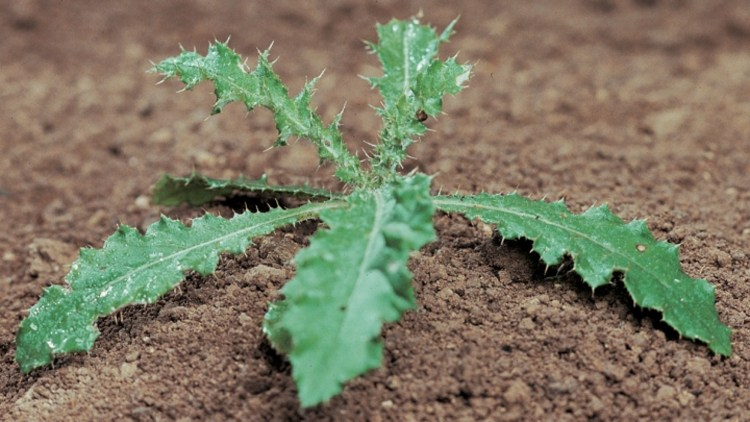
\includegraphics[width=\linewidth]{bench/img/adventice.jpg}
\end{center}
\end{minipage}

\vspace{0.2cm}

\begin{thebibliography}{10}
\beamertemplatearticlebibitems
\tiny
\bibitem{Buttazzo} G. Buttazzo, Can We Trust AI-Powered Real-Time Embedded
Systems? NG-RES (2022)
\end{thebibliography}

\end{frame}

\end{document}
